\documentclass[12pt]{article}

% ----------------------------------
% Language, encoding and fonts
% ----------------------------------
\usepackage[utf8]{inputenc}
\usepackage[T1]{fontenc}
\usepackage[english]{babel}
\usepackage{lmodern}
\renewcommand{\familydefault}{\sfdefault}
\usepackage{setspace}
\onehalfspacing
\setlength{\parskip}{6pt}
\setlength{\parindent}{0pt}
\usepackage[margin=1in]{geometry}
\usepackage{microtype}

% ----------------------------------
% Tables, figures, lists
% ----------------------------------
\usepackage{tabularx}
\usepackage{array}
\usepackage{booktabs}
\newcolumntype{L}[1]{>{\raggedright\arraybackslash}p{#1}}
\newcolumntype{Y}{>{\raggedright\arraybackslash}X}
\usepackage{graphicx}
\graphicspath{{figures/}}
\usepackage{float}
\usepackage[labelfont=bf]{caption}
\usepackage{enumitem}
\setlist{itemsep=0.5ex, topsep=0.5ex, parsep=0.5ex}
\usepackage{xcolor}
\definecolor{sectionblue}{RGB}{0,76,153}
\usepackage{sectsty}
\sectionfont{\color{sectionblue}\large\bfseries\sffamily}
\subsectionfont{\color{sectionblue}\normalsize\bfseries\sffamily}
\subsubsectionfont{\color{sectionblue}\normalsize\sffamily}

% ----------------------------------
% Mathematics
% ----------------------------------
\usepackage{amsmath, amssymb, amsthm, bm}
\DeclareMathOperator{\logit}{logit}
\newtheorem{proposition}{Proposition}
\newcommand{\code}[1]{\texttt{\small #1}}
% Expandable input, safe before \bottomrule inside tabular environments.
\makeatletter\newcommand{\tableinput}[1]{\@@input #1 }\makeatother

% ----------------------------------
% Citations and links
% ----------------------------------
\usepackage[authoryear,round]{natbib}
\usepackage[colorlinks, citecolor=blue, urlcolor=blue, linkcolor=blue, bookmarks=true]{hyperref}

% Structure note. Motivation and literature, data, model, estimation,
% identification, results, limitations, conclusions. Identification comes before
% the results because it explains why the relative-earnings observable, and not
% the aggregates, determines the level of the informal share.

\title{Measuring Colombia's Informal Output:\\
Relative Earnings and Identification in a Bayesian Two-Sector Model, 1993--2026}

\author{
  Jaime A. Vera-Jaramillo\thanks{Email: \href{mailto:jaimevera1107@gmail.com}{jaimevera1107@gmail.com},
  \href{mailto:ja.veraj@uniandes.edu.co}{ja.veraj@uniandes.edu.co};
  ORCID: \href{https://orcid.org/0000-0001-7611-6251}{0000-0001-7611-6251}}
}
\date{November 2026}

\begin{document}
\maketitle

\begin{abstract}
How much of Colombia's measured output is produced by informal work? The answer cannot be read from the labor-informality rate: Colombia combines an informality rate above 50\% with a much smaller informal share of output, because informal work is less productive. We estimate a Bayesian two-sector business-cycle model on quarterly national accounts and on reconstructed employment and informality series for 1993--2026. Identification comes from a new quarterly series of informal-to-formal labor earnings built from household-survey microdata for 2007--2026. Formal production uses capital and labor, informal production is labor based, and an accounting relationship maps relative earnings, the informality rate and the formal capital share into the informal output share. We show that aggregate data alone cannot pin down the size of the informal sector, and that relative earnings identify its quarterly path: from 2007 the path is invariant, within 0.3 percentage points, to the model's steady state. The informal share declines from about 30\% of GDP in 1993 to 20\% in 2026Q2, while labor informality falls from about 69\% to 54\%. The estimates lie within the range of published shadow-economy series for Colombia, close to the enhanced MIMIC estimates of Asllani, Dell'Anno and Schneider for 2009--2020. Sensitivity analysis quantifies the role of the capital share and of non-wage labor costs.
\end{abstract}

\noindent\textbf{Keywords:} informal output; labor informality; Bayesian DSGE; identification; relative earnings; Colombia

\noindent\textbf{JEL:} E26, E32, C11, O17

\section{Introduction}
\label{sec:introduction}

An economy can have a high proportion of informal workers without producing an equally high proportion of its output informally. The distinction is particularly consequential for Colombia. The national household-survey series used in this paper places labor informality at approximately 54\% of employment in 2026. Yet the relative productivity of work performed in small, unregistered, or own-account activities differs from that of registered wage employment. Translating a headcount into a share of value added requires information about those differences and a definition of what constitutes informal production.

The available indicators measure different objects. Labor informality counts \emph{workers}; DANE's multidimensional business-informality indicator counts \emph{establishments} and reported 90.2\% of microbusinesses as informal in 2024 \citep{DANE_IMIE}. The statistical office's estimate of the non-observed economy, 22.4\% of gross production in its 2015-base compilation, encompasses informal, underground and illegal activities as well as statistical adjustments \citep{DANE_SIECI}. The present study instead estimates the share of \emph{measured value added associated with informal work} under an explicit two-sector production model. These figures should not be equated: their units, denominators and coverage are different.

Dynamic general equilibrium (DGE) models are widely used to infer the size of the informal or shadow economy. Calibrated approaches fix its level at an external benchmark and model the subsequent dynamics \citep{ElginOztunali2012,SolisGarciaXie2017}. Bayesian DSGE approaches estimate latent sectoral activity jointly with structural shocks \citep{OrsiRaggiTurino2014}. Both require an identification argument, because aggregate observations alone do not always distinguish a large informal sector from a small one: different shares can be accommodated by changes in unobserved sectoral productivity and in the implied steady state. This paper supplies that argument with a direct measurement.

We investigate this problem with a deliberately parsimonious two-sector model. Competitive formal firms employ capital and labor; informal activities are represented by a labor-only technology, following a familiar strand of the literature \citep{IhrigMoe2004,ElginOztunali2012}. A household allocates work between the two activities, accumulates capital and chooses consumption. Aggregate shocks, a formality wedge and informal relative productivity generate business-cycle fluctuations. We estimate the model with a Kalman-filter likelihood and Bayesian Markov chain Monte Carlo methods. The macroeconomic data come from DANE's 2015-reference national accounts, with reconstructed quarterly observations before 2005. Total employment and labor informality are drawn from the GEIH-universe ICML series, which reconstructs the national labor market from 1993 \citep{VeraJaramillo2025ICML,VeraJaramillo2026Zenodo}.

The additional identifying information is a quarterly series of \emph{relative labor earnings}, constructed from DANE household-survey microdata since 2007. The ratio distinguishes worker groups and is adjusted for statutory non-wage employment costs on the formal side. Under the baseline production and measurement assumptions, the informal-to-formal output ratio equals the ratio of workers multiplied by relative value added per worker. The latter can be related to the survey earnings ratio and the formal capital share. This yields a transparent link between data and the quantity of interest (Proposition~\ref{prop:share}), in which every assumption is explicit and can be varied.

The paper makes four contributions. First, it provides a quarterly estimate of informal output for Colombia from 1993 to 2026, built on all the observed and reconstructed information available, together with the other quantities the model delivers: informal and formal GDP, relative productivity and the structural shocks behind them. Second, it shows through likelihood profiles, prior--posterior comparisons and simulations with known parameters that aggregate data alone do not determine the size of the informal sector, which explains why calibrated and estimated DGE models in the literature can reach very different levels. Third, it shows that relative earnings solve this problem for the object of interest: with them, the estimated \emph{path} of informal output is invariant to the model's steady-state share, and simulations recover the true share with high precision. Fourth, the data, code and diagnostics are public, so the series can be updated each quarter and re-estimated under alternative definitions, technologies and wage-cost conversions.

Under the preferred specification, informal work accounts for approximately 30.3\% of measured output in 1993 and 20.0\% in 2026Q2. The reduction parallels the decline in the labor-informality rate from approximately 69\% to 54\%; at the end of the sample, the implied informal value added per worker is about one-fifth of its formal counterpart. The estimate falls within the range of published Colombian shadow-economy estimates, close to the enhanced MIMIC series in 2009--2020 and to the Medina--Schneider series in 2008--2015 \citep{SchneiderBuehnMontenegro2010,MedinaSchneider2019,AsllaniDellAnnoSchneider2024,ElginKoseOhnsorgeYu2021}, although those series measure related but not identical concepts.

The paper is a measurement exercise: it reports the level of informal output together with the evidence and the accounting assumptions that determine it, so that each can be checked and improved.

The remainder of the paper reviews measurement approaches (Section~\ref{sec:background}), describes the data and their provenance (Section~\ref{sec:data}), presents the model and estimation (Sections~\ref{sec:model}--\ref{sec:estimation}), examines identification (Section~\ref{sec:identification}), and reports the estimates (Section~\ref{sec:results}). Section~\ref{sec:discussion} discusses their interpretation and Section~\ref{sec:limitations} the extensions that would sharpen them; Section~\ref{sec:conclusions} concludes.

\section{Background and related literature}
\label{sec:background}

\subsection{Measuring the informal economy}

The size of the informal or shadow economy cannot be observed directly, and the literature has developed several indirect approaches \citep{SchneiderEnste2000, MedinaSchneider2018}. Currency-demand methods attribute part of the demand for cash to transactions that avoid taxation or registration. For Colombia, \citet{ArangoMisasLopez2006} estimate the underground economy from 1976 to 2003 with a cash-demand function in state-space form. Multiple-indicators multiple-causes (MIMIC) models treat the shadow economy as a latent variable linked to causes such as taxation and regulation and to indicators such as currency and labor participation \citep{MedinaSchneider2018}. Panels for Colombia and most other countries are available from \citet{SchneiderBuehnMontenegro2010}, \citet{MedinaSchneider2019} and, with an enhanced MIMIC, \citet{AsllaniDellAnnoSchneider2024}; \citet{Vuletin2008} estimates the informal economy of Latin America and the Caribbean with a structural equation model, and the World Bank database of \citet{ElginKoseOhnsorgeYu2021} collects DGE and MIMIC estimates. These methods produce a time path but need an external value to fix its level, and their structural interpretation is limited.

Model-based approaches use the equilibrium conditions of an economy with a formal and an informal sector. \citet{IhrigMoe2004} and \citet{BusatoChiarini2004} study the allocation of labor between a taxed formal sector and an untaxed informal one. \citet{ElginOztunali2012} calibrate a two-sector dynamic general equilibrium model to produce shadow-economy estimates for many countries, fixing the level in a base year with an external estimate. \citet{SolisGarciaXie2017} show that the growth rate imposed on shadow productivity in that approach is not consistent with the model's balanced-growth conditions and derive it from the observed trends instead; the level is again fixed with an external base-year value. \citet{OrsiRaggiTurino2014} estimate an underground economy for Italy in a Bayesian DSGE model with limited tax enforcement; observed consumption, investment, tax revenues and regular earnings identify the latent sector, and the prior is centered on the official estimate of the statistical office. They note that a key parameter of the underground technology has a posterior almost identical to its prior.

\subsection{Informality in business-cycle models}

A second literature uses informality to explain business-cycle facts in emerging economies. \citet{RestrepoEchavarria2014} shows that if national accounts measure informal output incompletely, measured consumption is more volatile than measured output. \citet{FernandezMeza2015} estimate a model of informal employment for Mexico and find that informality is countercyclical and amplifies the response to productivity shocks. The stochastic trend of the present model follows \citet{AguiarGopinath2007}, who show that permanent productivity shocks account for much of the cycle in emerging economies.

\subsection{Identification}

Identification in DSGE models has been studied in general by \citet{CanovaSala2009}, \citet{Iskrev2010} and \citet{KoopPesaranSmith2013}. Bayesian estimation always delivers a posterior, so a parameter that the likelihood does not inform is reported with a posterior close to its prior. The present paper applies three standard checks to the parameter that matters for the measurement of the informal economy: the ratio of posterior to prior dispersion, the profile likelihood, and the recovery of a known value in simulated data.

\subsection{Official statistics in Colombia}

DANE publishes quarterly national accounts in volumes chained to the 2015 base. Its national accounts include an imputation for the non-observed economy, estimated at 22.4\% of total production in the 2015 base \citep{DANE_SIECI}; this concept refers to gross production, not value added, and includes underground, illegal and informal activities and statistical corrections. Labor informality is measured by the household survey (GEIH) and has changed definition over time; the ICML project reconstructs consistent national and territorial series from 1993 \citep{VeraJaramillo2025ICML}.

\section{Data}
\label{sec:data}

\subsection{Sources and provenance}

Table~\ref{tab:data} lists the series. The national accounts are quarterly volumes of the 2015 base, not seasonally adjusted. From 2005 they are the original DANE series; for 1993--2004 they are retropolated: GDP, consumption and investment by proportional disaggregation with seasonal profiles of the official series, and government consumption by the Denton--Cholette method \citep{Denton1971}. Employment and the informality rate come from the GEIH universe of ICML release 2.6.1 \citep{VeraJaramillo2025ICML, VeraJaramillo2026Zenodo}, aggregated from monthly to quarterly values. The informality rate is informal employment over total employment, consistent with the employment series by construction.

\begin{table}[H]
\centering
\caption{Observables and provenance.}
\label{tab:data}
\footnotesize
\begin{tabularx}{\textwidth}{L{3.6cm} L{3.7cm} Y}
\toprule
\textbf{Series} & \textbf{Source} & \textbf{Provenance by period} \\
\midrule
GDP, private consumption, gross fixed capital formation, government consumption & DANE quarterly national accounts, base 2015, chained volumes & 2005--2026: original series. 1993--2004: retropolated quarterly series. \\
Total employment & ICML 2.6.1, GEIH universe & 2001--2026: national survey (ECH and GEIH). 1993--2000: ICML reconstruction from annual survey levels of a different design. \\
Labor-informality rate & ICML 2.6.1, GEIH universe & 2021--2026: current definition. 2007--2020: inversion of published moving windows, with a bridge between definitions. 2001--2006: six aggregate anchors. 1993--2000: ICML backcast. \\
Relative labor earnings (informal / formal) & GEIH microdata, author's processing & 2007Q1--2026Q2, quarterly, by position and unit size; missing 2008Q2--Q4, 2011 and 2020Q2. Historical informality classification until 2021, current definition from 2022. \\
\bottomrule
\end{tabularx}
\end{table}

The provenance matters for the interpretation of the results. The quarterly dynamics of employment and informality before 2001 are generated by the ICML reconstruction, and the informality rate before 2007 is anchored to few observations. The estimation uses all quarters, which is the purpose of the reconstruction; Section~\ref{sec:identification} reports how much of the information about the size of the informal sector comes from each period.

\subsection{Relative labor earnings}

The earnings series is built from the monthly GEIH microdata processed by the author (January 2007 to August 2026). Each employed person is classified as formal or informal with the same rules that underlie the informality series: a size-and-position proxy until 2021 and the social-security-based definition from 2022, with persons whose status cannot be determined left unclassified rather than imputed. For workers with positive labor income, excluding unpaid family workers, the monthly weighted sums of income and of persons are computed with the national expansion factor of the survey, and the quarterly ratio is the weighted mean income of informal workers divided by that of formal workers. Income is DANE's derived labor income (main and secondary jobs) from mid-2008 and the sum of the main-job wage or profit and secondary-job income before. An alternative ratio uses income per hour worked.

Because the labor-only accounting of Section~\ref{sec:model} treats informal income as value added, the series is also computed by group of worker. On average over 2007--2026, 68.6\% of paid informal workers are own-account workers or employers, 22.3\% are employees in units of up to five persons, 5.6\% are domestic employees and 3.4\% are employees of units with six or more persons; the size question (P6870 until 2021, P3069 afterwards) is answered by all employees. The interpretation of these earnings differs by employment position. Income of own-account workers and employers includes a mixed-income component, whereas an employee's wage captures labor compensation but not the enterprise's entire value added. The baseline uses a group-specific \emph{proxy} for informal value added per worker: reported income for the first three groups and the wage divided by $1-\alpha$ for employees of larger units, who are assumed to work with the firm's capital. In particular, treating earnings of domestic workers and employees of small units as their entire attributable value added is an identifying approximation, not an accounting identity observed in the survey. The resulting proxy is divided by the mean wage of formal employees; formal own-account workers are excluded from the denominator because their income is not a wage. This adjustment changes the sample-average ratio from 0.421 (unadjusted) to 0.441. Section~\ref{sec:limitations} discusses its limitations.

The survey asks wage earners for their pay ``before deductions'', so the employee's own contributions are included in the reported wage. The difference between the reported wage and the employer's total labor cost, which is what the model's gross formal wage $(1-\alpha)Y_f/N_f$ measures, consists of the employer's social-security contributions, the payroll contributions (\emph{parafiscales}) and the social benefits paid outside the monthly wage. These are set by law and are computed quarter by quarter for a worker earning less than ten minimum wages: pension (employer share 11.6\% in 2007 and 12\% from 2008), health (8.5\%), occupational risk (0.5\%), family compensation fund (4\%), the payroll contributions to SENA and ICBF (5\%), and the benefits (service bonus, severance pay and its interest, and holidays, 21.8\%). The 2012 tax reform (Law 1607) removed the SENA and ICBF contributions from May 2013 and the employer's health contribution from January 2014 for these workers. Non-wage costs therefore fall from 51.9\% of the wage in 2008--2012 to 38.4\% from 2014. Let $d_t^{\mathrm{nw}}$ be the employer non-wage cost premium relative to the reported wage. Its log gross-up, $\ln(1+d_t^{\mathrm{nw}})$, converts the reported formal wage into labor cost in the measurement equation of Section~\ref{sec:identification}; a sensitivity uses contributions only, for the case in which reported income already includes the benefits.

The ratio is stable between 0.42 and 0.47 from 2007 to 2019, falls during the pandemic and drops to about 0.37 when the current definition of informality is introduced in 2022 (Figure~\ref{fig:earnings}). The drop coincides with the change of definition, when the share of unclassified workers falls from about 3.5\% to almost zero, and is treated as a level shift in the measurement equation. Twenty-one months of 2008 and 2011 lack a usable expansion factor in the normalized files and are missing, as are March and April 2020, when telephone collection left a quarter of the employed without a formality status; quarters require three valid months.

\begin{figure}[H]
\centering
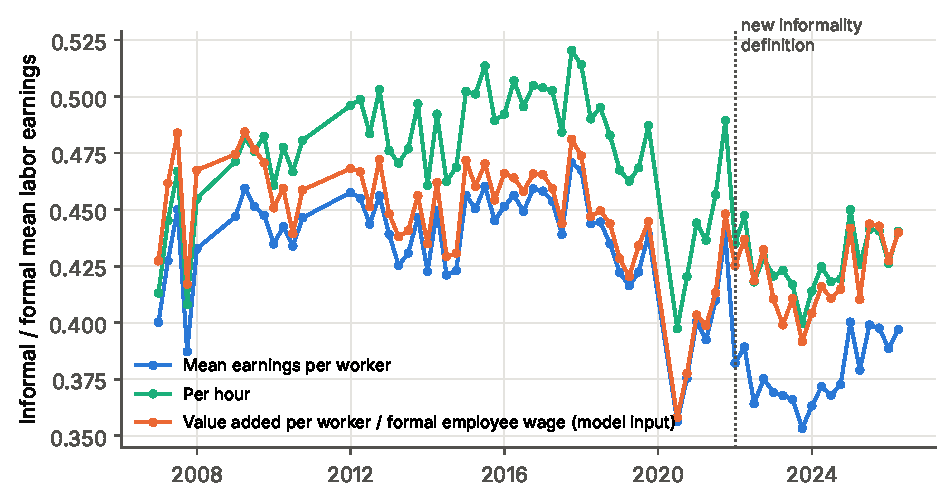
\includegraphics[width=0.85\textwidth]{fig_earnings.pdf}
\caption{Ratio of mean labor earnings of informal to formal workers, GEIH, 2007Q1--2026Q2. The dotted line marks the change in the definition of informality.}
\label{fig:earnings}
\end{figure}

\subsection{Transformations}

Let $Y_t$, $C_t$, $I_t$, $G_t$ and $N_t$ denote the levels and $s_t$ the informality rate. The observables are
\begin{equation}
\bm{y}^{\mathrm{obs}}_t = \big(\Delta\ln Y_t,\ \Delta\ln C_t,\ \Delta\ln I_t,\ \Delta\ln G_t,\ \Delta\ln N_t,\ \Delta\logit s_t\big)^{\top} - \bm{m}_{q(t)},
\label{eq:obs}
\end{equation}
where $\bm{m}_{q}$ is the mean of each growth rate in quarter of the year $q\in\{1,2,3,4\}$ over 2005--2018. Removing quarter-specific means removes deterministic seasonality and the mean growth rate together; the same means are applied to the whole sample. The earnings ratio enters in logarithmic \emph{levels}, $\ln R_t$, because its level is what identifies relative productivity. In the labor-only estimates the logit informality rate also enters in levels, as a deviation from the logit of its sample mean with the quarter-of-year pattern of 2005--2018 removed (Section~\ref{sec:identification}). The sample runs from 1993Q2 to 2026Q2 (133 quarters). The quarters 2020Q2--2020Q4, spanning the unprecedented contraction in output and employment and a change in survey collection mode, are treated as missing in the likelihood. The choice avoids asking a first-order Gaussian approximation to accommodate those exceptional observations, but it also means that the paper does not estimate the pandemic adjustment mechanism.

Two features of the data shape the estimation. First, quarterly growth rates have almost no persistence: excluding the pandemic quarters, the first-order autocorrelation is $-0.13$ for GDP, $0.06$ for consumption and $-0.21$ for employment, so no model can predict them much better than their mean. Second, the growth of investment and of the logit informality rate is negatively autocorrelated ($-0.45$ and $-0.37$), the signature of noise in levels.

\section{Model}
\label{sec:model}

The model is a standard real business-cycle economy with two ways of producing: a formal sector that uses capital and registered labor, and an informal sector made of own-account work and small units that uses labor only. It is kept as close as possible to the textbook structure so that the identification results are not driven by ad hoc features. This section derives every equilibrium condition from the optimization problems of households and firms, explains what each condition means, and shows how the informal share of output follows from them. The stationary system that is solved numerically, the steady-state algorithm and the linear solution are collected in Appendix~\ref{app:model}.

\subsection{Overview and notation}

Time is quarterly. The economy has a representative household, competitive formal firms, informal production units owned and run by the household, and a government. Table~\ref{tab:notation} lists the main symbols. Capital letters denote levels that grow with the economy; the corresponding lowercase letters, used from Section~\ref{sec:steady} on, denote the same variables divided by the trend.

\begin{table}[H]
\centering
\caption{Main notation.}
\label{tab:notation}
\footnotesize
\begin{tabularx}{\textwidth}{l X}
\toprule
\textbf{Symbol} & \textbf{Meaning} \\
\midrule
$C_t, I_t, G_t$ & Private consumption, investment, government consumption \\
$K_t$ & Capital stock available in quarter $t$ (all capital is used by formal firms) \\
$N_{f,t}, N_{i,t}$ & Formal and informal work \\
$s_t = N_{i,t}/(N_{f,t}+N_{i,t})$ & Labor-informality rate \\
$Y_{f,t}, Y_{i,t}, Y_t$ & Formal, informal and total output, $Y_t = Y_{f,t}+Y_{i,t}$ \\
$\theta_t = Y_{i,t}/Y_t$ & Informal share of output; $\theta$ without subscript is its steady state \\
$w_{f,t}, r_t$ & Formal wage and rental rate of capital \\
$\tau_t$ & Formality wedge on formal labor income (taxes, contributions, compliance costs) \\
$X_t$ & Labor-augmenting technology, common to both sectors, with a unit root \\
$R_t$ & Informal income per worker relative to the gross formal wage \\
$\alpha$ & Capital share of formal output \\
$\eta$ & Elasticity of informal output to informal work ($0<\eta<1$) \\
$\varphi$ & Inverse Frisch elasticity of labor supply \\
$\mu_t, z^g_t, \nu_t, \psi_t, \omega_t, x_t, z^r_t$ & Shocks: trend growth, government, investment efficiency, labor supply, wedge, absorption, informal productivity \\
\bottomrule
\end{tabularx}
\end{table}

\subsection{Household}
\label{sec:household}

\paragraph{Preferences.} A representative household chooses consumption, investment, next quarter's capital and the hours supplied to each sector to maximize expected lifetime utility
\begin{equation}
E_0 \sum_{t=0}^{\infty}\beta^t\Big[\ln C_t - \psi_t\,\frac{\chi_f N_{f,t}^{1+\varphi} + \chi_i N_{i,t}^{1+\varphi}}{1+\varphi}\Big].
\label{eq:utility}
\end{equation}
The first term is the satisfaction from consumption; the logarithm makes the marginal value of an extra peso fall as consumption rises. The second term is the disutility of work. Each type of work has its own convex cost: the hundredth hour in the informal sector is more costly than the first, and the same holds for formal work. This is the simplest specification in which the household supplies both types of work at the same time, as Colombian households do, instead of moving everybody to whichever sector pays slightly more. The weights $\chi_f$ and $\chi_i$ capture fixed differences in the attractiveness of the two sectors (access, flexibility, preferences) and are calibrated so that the model reproduces the mean informality rate. The shock $\psi_t$ shifts the disutility of all work (labor supply), $\beta$ is the discount factor and $1/\varphi$ is the Frisch elasticity of labor supply.

\paragraph{Budget and capital accumulation.} Each quarter the household receives formal wages net of the wedge, the whole output of the informal units it runs, the rental income of its capital, lump-sum transfers $T_t$ and an aggregate net-external-absorption transfer $B_t$, which is taken as given in the household optimization. It spends on consumption and investment:
\begin{equation}
C_t + I_t = (1-\tau_t)\,w_{f,t}N_{f,t} + Y_{i,t} + r_t K_t + T_t + B_t .
\label{eq:budget}
\end{equation}
Investment becomes capital with an efficiency that varies over time,
\begin{equation}
K_{t+1} = (1-\delta)K_t + \nu_t I_t ,
\label{eq:capital}
\end{equation}
where $\delta$ is depreciation and $\nu_t$ is a shock to the marginal efficiency of investment: a peso invested produces more or less new capital depending on financial conditions or the relative price of capital goods. The formality wedge is
\begin{equation}
1-\tau_t = (1-\bar\tau)\,e^{-\omega_t},
\label{eq:wedge}
\end{equation}
so that $\bar\tau$ is its steady-state level and an increase in $\omega_t$ makes formal work less attractive. The wedge summarizes everything that separates what a formal job costs from what the worker keeps: social-security contributions, payroll taxes and the costs of registration and compliance.

\paragraph{First-order conditions.} Let $\lambda_t$ be the Lagrange multiplier of the budget constraint (the marginal utility of a peso) and $\lambda_tq_t$ that of the capital accumulation equation (the value of a unit of installed capital). The Lagrangian is
\begin{multline}
\mathcal{L} = E_0\sum_{t=0}^{\infty}\beta^t\Big\{\ln C_t - \psi_t\frac{\chi_fN_{f,t}^{1+\varphi}+\chi_iN_{i,t}^{1+\varphi}}{1+\varphi}
+ \lambda_t\big[(1-\tau_t)w_{f,t}N_{f,t} + Y_{i,t} + r_tK_t + T_t + B_t - C_t - I_t\big] \\
+ \lambda_tq_t\big[(1-\delta)K_t + \nu_tI_t - K_{t+1}\big]\Big\}.
\end{multline}
Differentiating with respect to each choice and setting the derivative to zero gives five conditions.
\begin{align}
C_t:&\quad \lambda_t = \frac{1}{C_t}, \label{eq:foc-c}\\
I_t:&\quad q_t = \frac{1}{\nu_t}, \label{eq:foc-i}\\
K_{t+1}:&\quad \lambda_tq_t = \beta E_t\big[\lambda_{t+1}\big(r_{t+1} + q_{t+1}(1-\delta)\big)\big], \label{eq:foc-k}\\
N_{f,t}:&\quad \psi_t\chi_fN_{f,t}^{\varphi} = \lambda_t(1-\tau_t)w_{f,t}, \label{eq:foc-nf}\\
N_{i,t}:&\quad \psi_t\chi_iN_{i,t}^{\varphi} = \lambda_t\,\frac{\partial Y_{i,t}}{\partial N_{i,t}} . \label{eq:foc-ni}
\end{align}
Each has a direct reading. \eqref{eq:foc-c}: the value of a peso is the extra utility of consuming it. \eqref{eq:foc-i}: a unit of capital costs $1/\nu_t$ pesos of investment, so that is its price. \eqref{eq:foc-k}: the household gives up a unit of capital today, worth $\lambda_tq_t$, only if it expects to recover the same value tomorrow from the rent $r_{t+1}$ plus the undepreciated capital, discounted by $\beta$. Substituting \eqref{eq:foc-c} and \eqref{eq:foc-i} gives the Euler equation
\begin{equation}
\frac{1}{\nu_t C_t} = \beta E_t\Big[\frac{1}{C_{t+1}}\Big(r_{t+1} + \frac{1-\delta}{\nu_{t+1}}\Big)\Big].
\label{eq:euler}
\end{equation}
The two labor conditions say that the household works in each sector until the utility cost of the last hour equals the utility value of what that hour produces. Using \eqref{eq:foc-c} to replace $\lambda_t$,
\begin{equation}
\psi_t\chi_f N_{f,t}^{\varphi} C_t = (1-\tau_t)\,w_{f,t}, \qquad \psi_t\chi_i N_{i,t}^{\varphi} C_t = \frac{\partial Y_{i,t}}{\partial N_{i,t}} .
\label{eq:foc-labor}
\end{equation}
The left-hand side is the marginal rate of substitution between leisure and consumption: how many pesos of consumption the household asks for to work one more hour. The right-hand side is what that hour pays: the formal wage after the wedge in one case, the marginal product of informal work in the other. A higher wedge lowers the right-hand side of the formal condition, so the household shifts hours towards informal work until both conditions hold again.

\subsection{Formal firms}

Formal firms are competitive, rent capital from the household and hire formal work to produce with a Cobb--Douglas technology,
\begin{equation}
Y_{f,t} = K_t^{\alpha}\big(X_tN_{f,t}\big)^{1-\alpha}.
\label{eq:technology}
\end{equation}
A firm maximizes profits $Y_{f,t} - w_{f,t}N_{f,t} - r_tK_t$, which gives
\begin{equation}
r_t = \alpha\,\frac{Y_{f,t}}{K_t}, \qquad w_{f,t} = (1-\alpha)\,\frac{Y_{f,t}}{N_{f,t}} .
\label{eq:foc-firm}
\end{equation}
Each factor is paid its marginal product. Because the technology has constant returns, the payments exhaust output: a share $\alpha$ goes to capital and a share $1-\alpha$ to formal labor. This is the property used to estimate $\alpha$ (Section~\ref{sec:alpha}), and it is what makes the formal wage measured in the survey a fraction $1-\alpha$ of formal value added per worker.

Labor-augmenting technology has a unit root with stochastic growth \citep{AguiarGopinath2007},
\begin{equation}
\ln X_t - \ln X_{t-1} = \gamma + \mu_t ,
\label{eq:trend}
\end{equation}
so a shock $\mu_t$ shifts the level of productivity permanently. This is the standard way to represent the persistent swings in growth of emerging economies, and it means that output, consumption, investment and capital share a common stochastic trend.

\subsection{Informal production}

Following the shadow-economy literature \citep{IhrigMoe2004, ElginOztunali2012}, informal production uses labor only, with decreasing returns:
\begin{equation}
Y_{i,t} = A_i\,e^{z^r_t}\,X_t\,N_{i,t}^{\eta}, \qquad 0<\eta<1 .
\label{eq:informal-technology}
\end{equation}
$A_i$ is the level of informal productivity, $z^r_t$ a shock to it, and $X_t$ enters so that informal output grows with the economy. Decreasing returns ($\eta<1$) mean that each additional informal worker adds less than the previous one: informal activities compete for the same customers and spaces, and they cannot be scaled up without capital.

\paragraph{Average and marginal product.} The informal unit is run by the household, so there is no separate informal wage. Two quantities matter and must be kept apart:
\begin{equation}
\underbrace{\frac{Y_{i,t}}{N_{i,t}}}_{\text{average product: income per informal worker}}
\qquad\text{and}\qquad
\underbrace{\frac{\partial Y_{i,t}}{\partial N_{i,t}} = \eta\,\frac{Y_{i,t}}{N_{i,t}}}_{\text{marginal product: return of one more hour}} .
\label{eq:avg-marginal}
\end{equation}
The marginal product enters the household's choice of hours in \eqref{eq:foc-labor}. The average product is the latent value added per worker that the measurement exercise seeks to approximate with survey earnings. It is not automatically equal to every respondent's reported wage or profit.

\paragraph{Why labor only.} The justification is not that informal units use no capital, but what the household survey measures. The income reported by own-account workers and informal employers is mixed income or profit: it already contains the return to the vehicles, tools and premises of their own unit, and the wages they pay are counted in the income of their employees. Informal survey income is therefore a measure of informal value added per worker. The income of formal wage employees, by \eqref{eq:foc-firm}, represents only the labor share of formal value added. The labor-only technology implements these measurement conventions \emph{inside the model}: informal income per worker is defined as informal output per worker, whereas the formal wage is a fraction $1-\alpha$ of formal output per worker. Employees of informal units are the one group whose reported wage does not contain the unit's surplus, and the earnings series is adjusted for them by group (Section~\ref{sec:data}); alternative treatments are reported in the sensitivity analysis.

\subsection{Government, resources and shocks}

Government consumption is exogenous and grows with the trend, $G_t = \bar g\,X_t\,e^{z^g_t}$, and the government budget is balanced with lump-sum transfers, $T_t = \tau_tw_{f,t}N_{f,t} - G_t$. The wedge is therefore modeled as a transfer between agents, not a direct loss of resources; it changes the allocation of work. To account for national-account components outside the domestic three-good model, let $B_t=(\bar x+x_t)Y_t$ denote a reduced-form net transfer financing excess domestic absorption (or, when negative, net resources supplied to the rest of the world). It is taken as given by individual households. This is an accounting closure rather than a structural model of an external sector. Aggregating the household and government budgets and using \eqref{eq:foc-firm} gives
\begin{equation}
Y_t\,\big(1 + \bar x + x_t\big) = C_t + I_t + G_t .
\label{eq:resources}
\end{equation}
The term $\bar x+x_t$ represents omitted absorption and the statistical discrepancy arising from chained volumes. In particular, $Y=C+I+G$ is not a valid identity for Colombia's open economy or for non-additive chained-volume components. The steady-state term $\bar x$ reproduces the sample expenditure ratios; $x_t$ absorbs fluctuations in the omitted components. Because $B_t$ has no intertemporal law of repayment, this closure must not be interpreted as a structural theory of trade, external debt or fiscal financing.

The seven exogenous processes are independent first-order autoregressions,
\begin{equation}
\zeta_t = \rho_\zeta\,\zeta_{t-1} + \sigma_\zeta\,\varepsilon_{\zeta,t},\qquad \varepsilon_{\zeta,t}\sim N(0,1),\qquad \zeta\in\{\mu,\, z^g,\, \ln\nu,\, \ln\psi,\, \omega,\, x,\, z^r\},
\label{eq:shocks}
\end{equation}
with persistence $\rho_\zeta$ and volatility $\sigma_\zeta$. Their roles are distinct: $\mu$ moves the growth of productivity, $z^g$ government spending, $\nu$ the efficiency of investment, $\psi$ the willingness to work, $\omega$ the cost of formality, $x$ absorption and $z^r$ informal productivity. The informal-productivity shock is active only when the earnings observable of Section~\ref{sec:identification} is used; without it nothing in the data separates it from the wedge, and it is switched off in the estimates based on aggregates only.

\paragraph{Equilibrium.} An equilibrium is a set of quantities and prices that satisfy the household conditions \eqref{eq:capital}, \eqref{eq:euler} and \eqref{eq:foc-labor}, the firm conditions \eqref{eq:foc-firm}, the technologies \eqref{eq:technology} and \eqref{eq:informal-technology}, the resource constraint \eqref{eq:resources} and the laws of motion of the shocks. After substituting prices, the model has six endogenous variables ($C$, $Y$, $I$, $N_f$, $N_i$, $K$) and seven shocks, thirteen equations in total (Appendix~\ref{app:model}).

\subsection{The informal share of output}

\begin{proposition}[Informal share of output]
\label{prop:share}
Let $R_t$ be informal income per worker relative to the gross formal wage, $R_t \equiv (Y_{i,t}/N_{i,t})/w_{f,t}$, and $s_t \equiv N_{i,t}/(N_{f,t}+N_{i,t})$ the informality rate. Then
\begin{equation}
\theta_t \equiv \frac{Y_{i,t}}{Y_t} = \frac{(1-\alpha)\,R_t\,o_t}{1+(1-\alpha)\,R_t\,o_t},\qquad o_t\equiv\frac{s_t}{1-s_t}.
\label{eq:share}
\end{equation}
If instead both sectors shared the Cobb--Douglas technology with mobile capital, the factor $1-\alpha$ would disappear and $\theta_t$ would equal the informal share of labor income, $R_to_t/(1+R_to_t)$.
\end{proposition}

\emph{Proof.} Write the ratio of informal to formal output as a product of output per worker and workers:
\[
\frac{Y_{i,t}}{Y_{f,t}} = \frac{Y_{i,t}/N_{i,t}}{Y_{f,t}/N_{f,t}}\cdot\frac{N_{i,t}}{N_{f,t}}
= \frac{R_t\,w_{f,t}}{w_{f,t}/(1-\alpha)}\cdot o_t = (1-\alpha)\,R_t\,o_t ,
\]
where $o_t$ denotes the odds of informal employment and the second step uses the definition of $R_t$ and $w_{f,t}=(1-\alpha)Y_{f,t}/N_{f,t}$ from \eqref{eq:foc-firm}, and $N_{i,t}/N_{f,t}=s_t/(1-s_t)$. Then $\theta_t = (Y_{i,t}/Y_{f,t})/(1+Y_{i,t}/Y_{f,t})$. With a common technology both sectors have the same capital per efficiency unit of labor, output is proportional to labor income in each sector, and the factor $1-\alpha$ cancels. $\square$

Proposition~\ref{prop:share} is an accounting identity of the model, and it separates the measurement problem in three parts.
\begin{itemize}
  \item The informality rate $s_t$ is observed directly in the household survey.
  \item The earnings ratio $R_t$ is the object to identify. It is also measured in the survey, as the ratio of mean informal income to the mean wage of formal employees, after removing the wedge.
  \item The capital share $\alpha$ converts the formal wage into formal output per worker. It is estimated from the national accounts.
\end{itemize}
A numerical example shows how much each part matters. At an informality rate of 55\% ($o=1.22$) and $\alpha=0.35$, an earnings ratio of $R=0.2$ gives $\theta=14\%$ and $R=0.6$ gives $\theta=32\%$. With the same $R=0.35$, raising $\alpha$ from 0.35 to 0.50 lowers $\theta$ from 22\% to 18\%, and assuming equal technologies raises it to 30\%. For a fixed $R$ and $s$, the equal-technology expression is larger because it omits the factor $1-\alpha$. For given data it is therefore an upper bound.

\subsection{What moves the informality rate}

Dividing the two labor conditions in \eqref{eq:foc-labor} eliminates consumption and the labor-supply shock, which affect both sectors in the same way, and leaves the relative return of the two types of work:
\begin{equation}
\frac{\chi_i}{\chi_f}\Big(\frac{N_{i,t}}{N_{f,t}}\Big)^{\varphi} = \frac{\eta\,Y_{i,t}/N_{i,t}}{(1-\tau_t)(1-\alpha)\,Y_{f,t}/N_{f,t}} .
\label{eq:relative-return}
\end{equation}
The household moves work towards the informal sector when its marginal return rises relative to the after-wedge formal wage, and the convex costs ($\varphi>0$) limit how far it goes.

\begin{proposition}[Determinants of the informality rate]
\label{prop:rate}
Taking logarithms of \eqref{eq:relative-return}, with $Y_{i,t}/N_{i,t} = A_ie^{z^r_t}X_tN_{i,t}^{\eta-1}$,
\begin{equation}
\varphi\logit s_t + (1-\eta)\ln N_{i,t} + \ln\frac{Y_{f,t}}{X_tN_{f,t}}
= \ln\frac{\chi_f\,\eta A_i}{\chi_i\,(1-\alpha)} - \ln(1-\bar\tau) + z^r_t + \omega_t .
\label{eq:rate-labor-only}
\end{equation}
The right-hand side contains only the wedge and informal productivity. The left-hand side contains, besides the informality rate, the scale of informal work and formal output per efficiency unit of labor, which depends on capital per formal worker. Aggregate shocks to productivity, investment efficiency, labor supply, government spending or absorption therefore move the informality rate only through capital per formal worker and through the scale of informal employment. With equal technologies those two terms disappear and
\begin{equation}
\varphi\,\logit s_t = \ln\frac{\chi_f}{\chi_i} - \ln(1-\bar\tau) + \ln\tilde\rho + z^r_t + \omega_t ,
\label{eq:rate}
\end{equation}
so aggregate shocks do not move the informality rate at all.
\end{proposition}

\emph{Proof.} Take logarithms of \eqref{eq:relative-return}, use $N_{i,t}/N_{f,t} = s_t/(1-s_t)$, $\ln[s_t/(1-s_t)]=\logit s_t$ and \eqref{eq:wedge}, and collect the endogenous terms on the left. With equal technologies $Y_t=K_t^{\alpha}(X_tL_t)^{1-\alpha}$, $L_t = N_{f,t}+\tilde\rho e^{z^r_t}N_{i,t}$, the informal wage is $\tilde\rho e^{z^r_t}w_{f,t}$ and the ratio of wages does not depend on capital or on the scale of either sector. $\square$

Proposition~\ref{prop:rate} has a direct empirical consequence: the variance of the informality rate is attributed mostly to the formality wedge and to informal productivity (Section~\ref{sec:results}). It is also the reason why the informality rate carries little information about $R_t$ beyond its own level.

\paragraph{Equal technologies.} For comparison and as an upper bound, the model is also estimated with a common Cobb--Douglas technology, $Y_t=K_t^{\alpha}(X_tL_t)^{1-\alpha}$ with $L_t=N_{f,t}+\tilde\rho e^{z^r_t}N_{i,t}$, mobile capital and an informal wage $\tilde\rho e^{z^r_t}w_{f,t}$, where $\tilde\rho$ is the relative productivity of informal work. In that case $R_t = \tilde\rho e^{z^r_t}$ and the share of output equals the share of labor income.

\subsection{Trend, steady state and solution}
\label{sec:steady}

\paragraph{Removing the trend.} Output, consumption, investment, government consumption and capital grow with $X_t$, so they have no constant steady state. The model is made stationary by dividing them by the trend: $y_t=Y_t/X_t$, $c_t=C_t/X_t$, and so on, and $k_t=K_t/X_{t-1}$ for capital, which is chosen one quarter in advance. Work and the informality rate are already stationary. The stationary equations are listed in Appendix~\ref{app:model}.

\paragraph{Steady state.} With all shocks at zero the stationary model has a steady state that can be computed in closed form, step by step, for given $\theta$:
\begin{enumerate}[leftmargin=*]
  \item The Euler equation \eqref{eq:euler} with constant consumption growth $e^{\gamma}$ gives the rental rate, $r = e^{\gamma}/\beta - 1 + \delta$. With the calibration of Section~\ref{sec:estimation} it is 3.5\% per quarter.
  \item The firm condition \eqref{eq:foc-firm} gives the capital--output ratio of the formal sector, $K/Y_f = \alpha/r$: 10.0 quarters, or 2.5 years, close to the 2.4--2.8 measured by DANE for the whole economy.
  \item Hours are split according to the mean informality rate: $N_f = \bar N(1-\bar s)$ and $N_i=\bar N\bar s$, with $\bar N$ a normalization.
  \item Formal output follows from the technology, $Y_f = (K/Y_f)^{\alpha/(1-\alpha)}N_f$ in detrended units, and total output from the informal share, $Y = Y_f/(1-\theta)$, so $Y_i=\theta Y$ and $A_i = Y_i/N_i^{\eta}$.
  \item Investment replaces depreciation and keeps capital growing with the trend, $I = (e^{\gamma}-1+\delta)\,\tilde K$ with $\tilde K = K_t/X_t$. The implied ratio $I/Y$ is 14\%, below the 19\% of the data, because the model has no residential or public investment of its own; consumption and government consumption are set at their sample ratios to GDP, and $\bar x$ closes the resource constraint.
  \item Finally, the weights $\chi_f$ and $\chi_i$ are those that make the labor conditions \eqref{eq:foc-labor} hold at the chosen $N_f$ and $N_i$.
\end{enumerate}
The last step is important for identification. Because $A_i$, $\chi_f$ and $\chi_i$ adjust, \emph{any} value of $\theta$ is consistent with the observed informality rate and with all steady-state ratios: the level of $\theta$ is not pinned down by the first moments of the aggregates. The same holds with equal technologies, where $\tilde\rho=\theta(1-\bar s)/[(1-\theta)\bar s]$. Whatever information there is about $\theta$ must come from dynamics or from an additional observable (Section~\ref{sec:identification}).

\paragraph{Solution.} The thirteen stationary equations are linearized around the steady state: each variable is replaced by its log deviation from the steady state, and each equation by its first-order Taylor approximation. The result is a linear system $\bm{A}\,E_t\bm{z}_{t+1} = \bm{B}\,\bm{z}_t$, in which eight variables are predetermined (capital and the seven exogenous processes) and the other five (consumption, output, investment and the two types of work) are choices that can jump when news arrives. The system is solved by the generalized Schur decomposition \citep{Klein2000}, which returns the unique stable solution
\begin{equation}
\bm{s}_{t+1} = \bm{T}\bm{s}_t + \bm{R}\bm{\varepsilon}_{t+1},\qquad \text{jumps}_t = \bm{P}\bm{s}_t ,
\label{eq:solution}
\end{equation}
where $\bm{s}_t$ collects the eight state variables (capital and the seven shocks). A unique stable solution exists when the number of stable eigenvalues equals the number of states (the Blanchard--Kahn condition); this is checked at every parameter draw, and draws that violate it get zero posterior density.

\section{Estimation}
\label{sec:estimation}

\subsection{State-space form}

Let $\bm{x}_t$ be the vector of predetermined variables of the linearized model (capital and the exogenous processes), with law of motion $\bm{x}_{t+1} = \bm{T}\bm{x}_t + \bm{R}\bm{\varepsilon}_{t+1}$, and let all model variables be $\bm{M}\bm{x}_t$. Each observable in \eqref{eq:obs} is a difference of model variables plus the trend shock for the variables with a trend, for example $\Delta\ln Y_t = \hat y_t - \hat y_{t-1} + \mu_t$. The state is therefore augmented with its lag.

Survey and statistical noise is modeled in \emph{levels}. For investment, employment and the logit informality rate, the observed log level equals the model level plus an independent error $e_{j,t}\sim N(0,\sigma^2_{e_j})$, so that the growth rate contains $e_{j,t}-e_{j,t-1}$. These errors are added as states. This specification produces the negative first-order autocorrelation of the corresponding growth rates and lets the Kalman smoother separate survey noise from movements in the latent informality rate. A small error with standard deviation $10^{-3}$ is added to every growth rate to keep the innovation covariance non-singular. The likelihood is evaluated with the Kalman filter, initialized at the unconditional distribution; quarters with missing observations skip the update step \citep{DurbinKoopman2012}. The implementation was checked against the exact Gaussian likelihood of the stacked observations. Appendix~\ref{app:model} writes every measurement equation explicitly and explains the filter and the sampler step by step.

\subsection{Calibration}

Table~\ref{tab:calibration} lists the parameters fixed before estimation. Those taken from the data are sample means of 1993--2026. The capital share and depreciation come from Colombian sources and from the data, as described below; the equal-technology estimates use $\alpha=0.33$, for which the depreciation implied by the investment ratio is also 4\% a year. The informal share $\theta$ is \emph{not} calibrated: it is estimated, and its steady state is recomputed at every draw. Section~\ref{sec:identification} shows that the object of interest, the path of the informal share, does not depend on its value.

\begin{table}[H]
\centering
\caption{Calibrated parameters.}
\label{tab:calibration}
\footnotesize
\begin{tabularx}{\textwidth}{L{1.6cm} L{6.2cm} r Y}
\toprule
\textbf{Parameter} & \textbf{Meaning} & \textbf{Value} & \textbf{Source} \\
\midrule
$\alpha$ & Capital share of formal output & 0.354 & Estimated, Section~\ref{sec:alpha} \\
$\beta$ & Quarterly discount factor & 0.985 & Conventional, emerging economy \\
$\varphi$ & Inverse Frisch elasticity & 1.0 & Conventional \\
$\bar\tau$ & Steady-state formality wedge & 0.25 & Affects only the scale of $\chi_f$ \\
$\gamma$ & Mean quarterly trend growth & 0.0096 & GDP, 2005--2018 \\
$\bar s$ & Mean informality rate & 0.645 & ICML, 1993--2026 \\
$C/Y$, $I/Y$, $G/Y$ & Expenditure ratios & 0.697, 0.186, 0.139 & National accounts, 1993--2026 \\
$\delta$ & Quarterly depreciation & 0.0102 & 4\% a year; GRECO 3.1\%, DNP 3.8\% \\
$\bar x$ & Chain-volume residual & -- & Implied by expenditure ratios \\
$\ln(1+d_t^{\mathrm{nw}})$ & Non-wage labor costs of formal employees & 0.42 / 0.32 & Statutory rates, 2008--2012 / 2014--; Section~\ref{sec:data} \\
\bottomrule
\end{tabularx}
\end{table}

\subsection{Capital share and depreciation}
\label{sec:alpha}

Depreciation is set at the standard 4\% a year. Colombian estimates are close: the capital stocks of the Banco de la Rep\'ublica growth project (GRECO), built with the method of \citet{Barrios1993}, imply 2\% for buildings, 5\% for machinery and equipment and 3.1\% for total fixed capital between 1950 and 1997 \citep{GRECO1999}, and the National Planning Department uses 3.8\% \citep{RodriguezPerillaReyes2004}.

The capital share of formal output is estimated. Capital is built by the perpetual-inventory method from gross fixed capital formation in constant prices, and
\begin{equation}
\ln\frac{Y_{f,t}}{N_{f,t}} = c + \alpha\ln\frac{K_t}{N_{f,t}} + g\,t + e_t
\label{eq:dols}
\end{equation}
is estimated by dynamic OLS \citep{StockWatson1993} with one lead and lag and Newey--West errors on annual data for 1993--2025. Formal output $Y_{f,t}=(1-\theta_t)Y_t$ and formal employment $N_{f,t}=(1-s_t)N_t$ depend on $\alpha$ through \eqref{eq:share}, so $\alpha$ is a fixed point. With 4\% depreciation the estimate is 0.354 (standard error 0.25); it is 0.33 with 6\% and 0.30 with 8\%. The regression without trend gives 0.39--0.43, which absorbs productivity growth into capital, and the aggregate regression gives an implausible 0.65. The time series is short and the estimate is imprecise, but it is in the range of earlier Colombian estimates: GRECO finds 0.42 for 1925--1981 by cointegration and 0.36--0.41 for 1926--1994 and 1950--1994 by restricted least squares \citep{GRECO1999}, and the National Planning Department 0.39--0.51 depending on the specification \citep{RodriguezPerillaReyes2004}. Sensitivities with $\alpha=0.33$ (and 6\% depreciation) and $\alpha=0.50$ are reported in Section~\ref{sec:results}.

\subsection{Priors and sampler}

The estimated parameters are the informal share $\theta$, the labor elasticity of informal production $\eta$ (labor-only model), the seven persistences and seven innovation standard deviations (including the relative-productivity shock), the four measurement-error standard deviations (three level errors and the error of the earnings ratio) and the level shift $b$ of the earnings ratio from 2022Q1. Persistences, $\theta$ and $\eta$ have beta priors ($\eta$ with mean 0.7 and standard deviation 0.1), standard deviations inverse-gamma priors and $b$ a normal prior with mean zero and standard deviation 0.2 (Table~\ref{tab:posterior}). The prior of $\theta$, with mean 0.35 and standard deviation 0.10, is deliberately wide: its 90\% interval covers informal shares from about 19\% to 52\% of output.

The posterior is sampled in an unconstrained parameterization (logit for parameters in the unit interval, logarithm for standard deviations, identity for $b$), including the Jacobian. The posterior mode is found from three starting points by Nelder--Mead followed by BFGS; the inverse Hessian at the mode, computed by finite differences, is the proposal covariance of a random-walk Metropolis--Hastings sampler \citep{AnSchorfheide2007}. Eight chains start from over-dispersed points around the mode; during 15{,}000 burn-in iterations the proposal scale is adapted towards an acceptance rate of 0.28 \citep{RobertsGelmanGilks1997}, and 40{,}000 further iterations per chain are kept with a fixed proposal (four chains of 30{,}000 after 10{,}000 in the equal-technology and aggregates-only estimates). Convergence is assessed with the rank-normalized split $\hat R$ and the bulk and tail effective sample sizes of \citet{Vehtari2021}.

\section{Identification of the size of the informal sector}

This section uses the model without the earnings observable to show what aggregate data can say about the level of the informal share, and then introduces the observable that identifies it. The evidence is reported for the equal-technology model, where the mechanism is transparent; the labor-only technology does not change the conclusion (Section~\ref{sec:alt-tech}).
\label{sec:identification}

\subsection{Where information about the level can come from}

Section~\ref{sec:model} shows that steady-state ratios are consistent with any value of $\theta$. In the log-linearized equal-technology model, $\theta$ enters the dynamics only through the weights of the two types of work in effective labor,
\begin{equation}
d\ln L_t = (1-\theta)\,d\ln N_{f,t} + \theta\,d\ln N_{i,t},
\label{eq:effective}
\end{equation}
so the only source of information is the co-movement of output with the composition of employment. When the wedge moves workers between sectors, output changes more if informal work is much less productive than formal work (small $\theta$) and less if the two are similar (large $\theta$). This is a single, weak moment, and it is measured with noise because the informality rate itself is noisy (Section~\ref{sec:data}).

\subsection{Evidence}

Three checks are reported. Figure~\ref{fig:profiles} and Table~\ref{tab:profiles} show the profile log likelihood: for each fixed value of $\theta$ the other parameters are re-optimized and the maximized log likelihood is reported relative to its maximum. A drop of 1.92 is the conventional profile-likelihood reference corresponding to a one-parameter 95\% likelihood-ratio interval under regular identification. Because weak identification is precisely at issue here, the line is a descriptive benchmark rather than a formally calibrated test.

\begin{figure}[H]
\centering
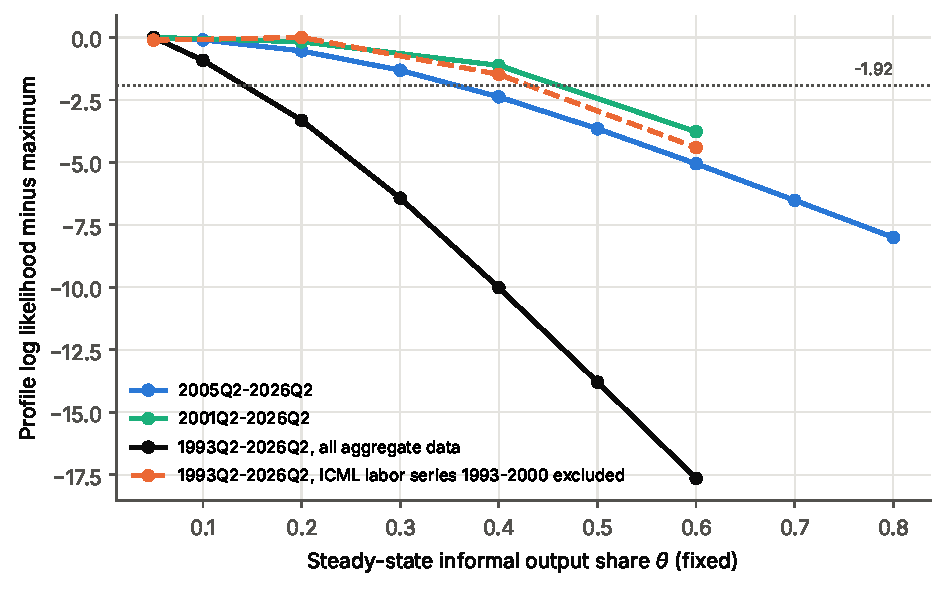
\includegraphics[width=0.85\textwidth]{fig_profiles.pdf}
\caption{Profile log likelihood of the steady-state informal share $\theta$, by sample. Values relative to the maximum of each profile; the dotted line marks $-1.92$.}
\label{fig:profiles}
\end{figure}

\begin{table}[H]
\centering
\caption{Profile log likelihood relative to its maximum.}
\label{tab:profiles}
\footnotesize
\begin{tabularx}{\textwidth}{Y rrrr}
\toprule
\textbf{Sample} & $\theta=0.05$ & $\theta=0.20$ & $\theta=0.40$ & $\theta=0.60$ \\
\midrule
1993Q2--2026Q2, all aggregate data & 0.00 & $-3.32$ & $-10.02$ & $-17.65$ \\
1993Q2--2026Q2, ICML informality 1993--2000 left out & 0.00 & $-3.93$ & $-13.82$ & $-18.76$ \\
1993Q2--2026Q2, ICML employment and informality 1993--2000 left out & $-0.11$ & 0.00 & $-1.48$ & $-4.41$ \\
2001Q2--2026Q2 & 0.00 & $-0.18$ & $-1.12$ & $-3.77$ \\
2005Q2--2026Q2 & 0.00 & $-0.54$ & $-2.38$ & $-5.06$ \\
\bottomrule
\end{tabularx}
\end{table}

With the full sample the likelihood is informative: it favors small informal shares and rejects values above about 0.15. The information comes from the 1993--2000 period, and specifically from the employment series. Leaving out the informality rate of those years does not change the profile; leaving out employment as well makes it nearly flat, as are the profiles of the samples that start in 2001 or 2005. In those samples the likelihood varies by less than 1.5 log points between $\theta=0.05$ and $\theta=0.40$, and it only begins to penalize the largest values.

The second check compares prior and posterior dispersion. With all aggregate data the posterior standard deviation of $\theta$ is 57\% of the prior one (median 0.18, 90\% interval 0.10--0.29), against 80\% when the 1993--2000 labor series are left out and 81\% in the 2005 sample.

The third check uses simulated data. The model is simulated at the posterior median of the 2005 sample with a true informal share of 0.45, ten points above the prior mean, over the same 85 quarters and with the same missing quarters, and re-estimated (posterior mode and Laplace standard deviation) in three replications. Table~\ref{tab:simulation} reports the results. With the six aggregates the estimate lies between 0.51 and 0.56, with a standard deviation of about 0.08, close to the prior's 0.10: the data do not recover the true value.

\begin{table}[H]
\centering
\caption{Recovery of a known informal share ($\theta=0.45$) in simulated data, 2005Q2--2026Q2.}
\label{tab:simulation}
\footnotesize
\begin{tabularx}{\textwidth}{Y rrr rrr}
\toprule
& \multicolumn{3}{c}{\textbf{Six aggregates}} & \multicolumn{3}{c}{\textbf{Plus relative earnings}} \\
\cmidrule(lr){2-4}\cmidrule(lr){5-7}
\textbf{Replication} & 1 & 2 & 3 & 1 & 2 & 3 \\
\midrule
Posterior mode of $\theta$ & 0.561 & 0.508 & 0.554 & 0.450 & 0.448 & 0.459 \\
Laplace standard deviation & 0.083 & 0.076 & 0.079 & 0.004 & 0.004 & 0.005 \\
Ratio to prior standard deviation & 0.83 & 0.76 & 0.79 & 0.04 & 0.04 & 0.05 \\
\bottomrule
\end{tabularx}
\end{table}

\subsection{Alternative technology}
\label{sec:alt-tech}

A frequent alternative in the shadow-economy literature lets the informal sector produce with labor only and decreasing returns, $Y_{i,t} = A_i X_t N_{i,t}^{\eta}$ \citep{IhrigMoe2004, ElginOztunali2012}. With that technology aggregate shocks change the relative return of the two types of work, and the informality rate responds to capital and to the trend shock. Estimated on the 2005 sample with $\eta$ free (prior mean 0.7), the profile likelihood of $\theta$ is as flat as with the common technology on the same sample: it falls by 2.1 log points between $\theta=0.10$ and $\theta=0.40$. A different technology does not solve the identification problem.

\subsection{An observable that identifies the level}

Proposition~\ref{prop:share} indicates what is missing: a direct measure of the earnings ratio $R_t$. In the labor-only model the observed ratio of informal income per worker to the mean wage of formal employees is
\begin{equation}
\ln R^{\mathrm{obs}}_t = \ln\frac{Y_{i,t}}{N_{i,t}} - \ln\Big((1-\alpha)\frac{Y_{f,t}}{N_{f,t}}\Big) + \ln(1+d_t^{\mathrm{nw}}) + b\,\mathbb{1}_{t\ge 2022Q1} + e^{R}_t,
\label{eq:earnings}
\end{equation}
where $\ln(1+d_t^{\mathrm{nw}})$ converts the wage reported by formal employees into the employer's labor cost using the statutory non-wage costs of Section~\ref{sec:data} (a constant wedge, $-\ln(1-\bar\tau)$ with $\bar\tau=0.25$, in a sensitivity), $b$ is a level shift for the change in the definition of informality and $e^{R}_t$ is measurement error. In log deviations the first two terms are $z^r_t + (\eta-1)\hat n_{i,t} - \alpha(\hat k_t - \mu_t - \hat n_{f,t})$, and their steady-state value is a function of $\theta$. With equal technologies the first two terms reduce to $\ln\tilde\rho + z^r_t$. The ratio can be computed from the household survey for every month since 2007 with the same classification of informality as the employment series. Equation \eqref{eq:earnings} enters the state space in levels and activates the shock $z^r_t$. In the simulation of Table~\ref{tab:simulation}, adding this observable recovers the true share with a standard deviation of half a percentage point.

In the labor-only model the earnings ratio depends on informal employment through $\eta$. If the informality rate entered only in changes, a very persistent deviation of the wedge could shift $\hat n_{i,t}$ and mimic a different $\theta$: in a first estimation the chains settled on different values of $\theta$ ($\hat R=1.57$). The labor-only estimates therefore observe the logit of the informality rate in levels, as a deviation from the logit of its sample mean with the quarter-of-year pattern removed, with an independent level error. This pins the state of the wedge in every quarter and removes the trade-off.

\subsection{Identification in the baseline model}
\label{sec:id-baseline}

Three checks are repeated for the baseline: the labor-only model with the informality rate in levels and the earnings observable.

\paragraph{Recovery of a known share.} Data are simulated from the baseline at its posterior median with a known steady-state share of 0.20 or 0.40, with the same length and missing quarters as the actual data, and $\theta$ is re-estimated (posterior mode and Laplace standard deviation) with and without the earnings observable (Table~\ref{tab:sim-labor-only}). Without earnings the estimate is roughly centered on the truth but its standard deviation is 41\%--46\% of the prior's. With earnings it is recovered within half a percentage point, with a standard deviation of 3\%--5\% of the prior's.

\begin{table}[H]
\centering
\caption{Recovery of a known steady-state share in data simulated from the baseline model (three replications per value).}
\label{tab:sim-labor-only}
\footnotesize
\begin{tabular}{c l c c c c}
\toprule
\textbf{True $\theta$} & \textbf{Observables} & \textbf{Mean mode} & \textbf{sd of modes} & \textbf{Laplace sd} & \textbf{Ratio to prior sd} \\
\midrule
\tableinput{tables/simulation_labor_only.tex}
\bottomrule
\end{tabular}
\end{table}

\paragraph{Profile likelihood in the data.} In the actual data the picture is different (Table~\ref{tab:profile-labor-only}). With or without earnings, the profile likelihood of the steady-state share is highest at the lowest value of the grid and falls monotonically. The likelihood alone does not pin down the steady state: the data can be matched with a low $\theta$ and with the economy away from its steady state for the whole sample, through levels that are not observed, such as the capital stock and total employment relative to their long-run values, which very persistent shocks can sustain. Observing the capital--output ratio built by perpetual inventory does not change this (Section~\ref{sec:results}).

\begin{table}[H]
\centering
\caption{Profile log likelihood of the steady-state share, baseline model with the constant wedge (relative to the maximum).}
\label{tab:profile-labor-only}
\footnotesize
\begin{tabular}{c c c}
\toprule
$\theta$ & \textbf{Aggregates only} & \textbf{With earnings ratio} \\
\midrule
\tableinput{tables/profile_labor_only.tex}
\bottomrule
\end{tabular}
\end{table}

\paragraph{What is identified: the path.} The quantity of interest is not the steady state but the informal share in each quarter, and Proposition~\ref{prop:share} shows that it depends on the informality rate and the earnings ratio of that quarter, both measured, and on $\alpha$. Table~\ref{tab:invariance} fixes the steady-state share at values between 0.10 and 0.40, re-optimizes every other parameter and recomputes the smoothed path. From 2007, when the earnings ratio is observed, the path changes by at most 0.3 percentage points; in the 1990s, where it is carried back by the model, by at most 1.4 points. Without the earnings observable nothing ties the path to a measured level, and the estimates without earnings are far from those with them (Section~\ref{sec:results}). The earnings ratio therefore identifies the level and trajectory of the output-share path. Before 2007 the path is identified with the information available for those years, the informality rate and the aggregates, and the model carries the earnings information back; the invariance table shows that this step moves the 1990s by at most 1.4 points. The steady-state parameter $\theta$ plays the role of a nuisance parameter: the likelihood does not pin it down on its own, its posterior combines the likelihood with the priors on the persistence of the shocks, and the path, which is the object of the paper, does not depend on it.

\begin{table}[H]
\centering
\caption{Informal share of output (\%) when the steady-state share is fixed and all other parameters are re-optimized, baseline model.}
\label{tab:invariance}
\footnotesize
\begin{tabular}{c c c c c c c}
\toprule
\textbf{Fixed $\theta$} & \textbf{1993Q2} & \textbf{2000Q4} & \textbf{2007Q2} & \textbf{2015Q2} & \textbf{2019Q2} & \textbf{2026Q2} \\
\midrule
\tableinput{tables/invariance.tex}
\bottomrule
\end{tabular}
\end{table}

Section~\ref{sec:results} applies the observable to the data.

\section{Results}
\label{sec:results}

The baseline estimate uses the labor-only informal sector, the statutory non-wage costs of formal employees and the available data from 1993Q2 to 2026Q2: the five aggregate growth rates, the level of the informality rate, including the ICML reconstruction of the labor market, and the value-added earnings ratio from 2007. The equal-technology estimate is reported as an upper bound and the estimate without earnings as a reference.

\subsection{Posterior and convergence}

Table~\ref{tab:posterior} reports the prior, the posterior median and 90\% interval, the ratio of posterior to prior standard deviation, and the convergence diagnostics. The largest rank-normalized $\hat R$ is 1.005, for $\theta$. The smallest bulk effective sample size is 1{,}718 and the smallest tail effective sample size 1{,}067, out of 320{,}000 retained draws; acceptance rates are between 0.23 and 0.30.

\begin{table}[H]
\centering
\caption{Prior and posterior distributions, baseline estimate (labor-only informal sector, statutory non-wage costs).}
\label{tab:posterior}
\scriptsize
\begin{tabular}{l l r c r r r}
\toprule
\textbf{Parameter} & \textbf{Prior (mean, sd)} & \textbf{Median} & \textbf{90\% interval} & \textbf{sd ratio} & $\hat R$ & \textbf{ESS} \\
\midrule
\tableinput{tables/posterior.tex}
\bottomrule
\end{tabular}
\end{table}

The steady-state informal share has a posterior median of 0.262 and a 90\% interval of 0.240--0.277; its posterior standard deviation is 12\% of the prior one, against 57\% when the earnings ratio is not observed (Figure~\ref{fig:prior-posterior}). As Section~\ref{sec:id-baseline} shows, this concentration owes part of its strength to the priors on the persistence of the shocks; the object identified by the data is the path of the share. The median earnings ratio is $R\approx0.31$: informal income per worker is about 31\% of the labor cost of a formal employee, and informal value added per worker, $(1-\alpha)R$, is about 20\% of formal value added per worker. The labor elasticity of informal production $\eta$ is not informed by the data (its posterior is the prior). The informal-productivity shock is persistent (0.92) and small (1.6\% per quarter), and the measurement error of the earnings ratio is 3.3\%. With formal employees in the denominator, the level shift of the earnings ratio in 2022 is small and not distinguishable from zero ($-0.035$, 90\% interval $-0.079$ to $0.009$).

\begin{figure}[H]
\centering
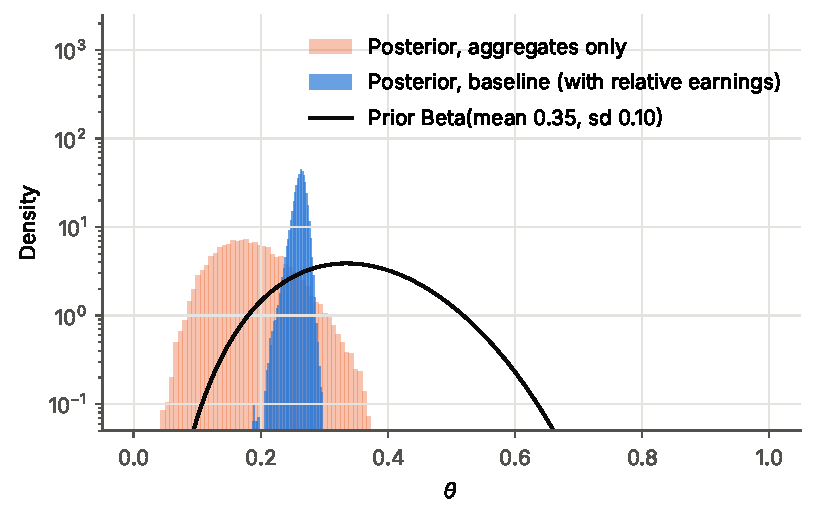
\includegraphics[width=0.75\textwidth]{fig_prior_posterior.pdf}
\caption{Prior and posteriors of the steady-state informal share $\theta$: baseline with the earnings observable and estimate with aggregates only (logarithmic density scale).}
\label{fig:prior-posterior}
\end{figure}

\subsection{Fit}

Table~\ref{tab:fit} compares the root mean squared one-step-ahead prediction error of the model with the standard deviation of each observable and with the error of a univariate first-order autoregression. Because quarterly growth rates have almost no persistence, the relevant benchmark is the autoregression. The model is within about three percent of it for GDP, consumption and employment, and improves on it for government consumption. The informality rate, now observed in levels, is predicted with an error of 15\% of its standard deviation, close to that of the autoregression.

\begin{table}[H]
\centering
\caption{One-step-ahead prediction, baseline estimate (pandemic quarters excluded).}
\label{tab:fit}
\footnotesize
\begin{tabular}{l r r r r}
\toprule
\textbf{Observable} & \textbf{sd} & \textbf{Autocorrelation} & \textbf{RMSE/sd, model} & \textbf{RMSE/sd, AR(1)} \\
\midrule
\tableinput{tables/fit.tex}
\bottomrule
\end{tabular}
\end{table}

\subsection{What drives informality}

Table~\ref{tab:variance} reports the forecast-error variance decomposition at the posterior median. The formality wedge explains most of the variance of the informality rate, from 67\% at one quarter to 92\% at twenty years, and informal productivity most of the rest. Unlike the equal-technology model, aggregate shocks now move the informality rate (Proposition~\ref{prop:rate}), but their contribution is small: the trend shock accounts for about 4\% at short horizons and investment efficiency and labor supply for about 2\% at long horizons. The informal output share is driven at short horizons by informal productivity (73\% at one quarter) and in the long run by the wedge (66\%). Detrended output is driven by the labor-supply shock and by the wedge, which moves workers between sectors with very different value added per worker.

\begin{table}[H]
\centering
\caption{Forecast-error variance decomposition at the posterior median (\%), baseline estimate.}
\label{tab:variance}
\scriptsize
\begin{tabular}{l r rrrrrrr}
\toprule
\textbf{Variable} & \textbf{Horizon} & \textbf{Trend} & \textbf{Gov.} & \textbf{Inv.\ eff.} & \textbf{Labor supply} & \textbf{Wedge} & \textbf{Absorption} & \textbf{Inf.\ prod.} \\
\midrule
\tableinput{tables/variance.tex}
\bottomrule
\end{tabular}
\end{table}

\subsection{The informal share of output, 1993--2026}

Figure~\ref{fig:share} shows the informal share of output computed from \eqref{eq:share} for 400 posterior draws, with the informality rate and the earnings ratio filtered by the Kalman smoother. The posterior median is 30.3\% of GDP in 1993 (90\% band in 1993Q2 28.8\%--31.2\%) and reaches its maximum, 30.7\%, in 1995. It is 29.7\% in 2000, 27.8\% in 2005 and 27.9\% in 2010, and then declines to 25.8\% in 2015, 23.4\% in 2019, 21.8\% in 2022 and 20.0\% in 2026Q2 (90\% band 19.4\%--20.7\%). The decline of ten percentage points follows that of the informality rate, from 69\% to 54\% of the employed; the earnings ratio adds quarterly variation but no trend. The equal-technology estimate is eight to eleven points higher, and the estimate without earnings seven to nine points lower.

\begin{figure}[H]
\centering
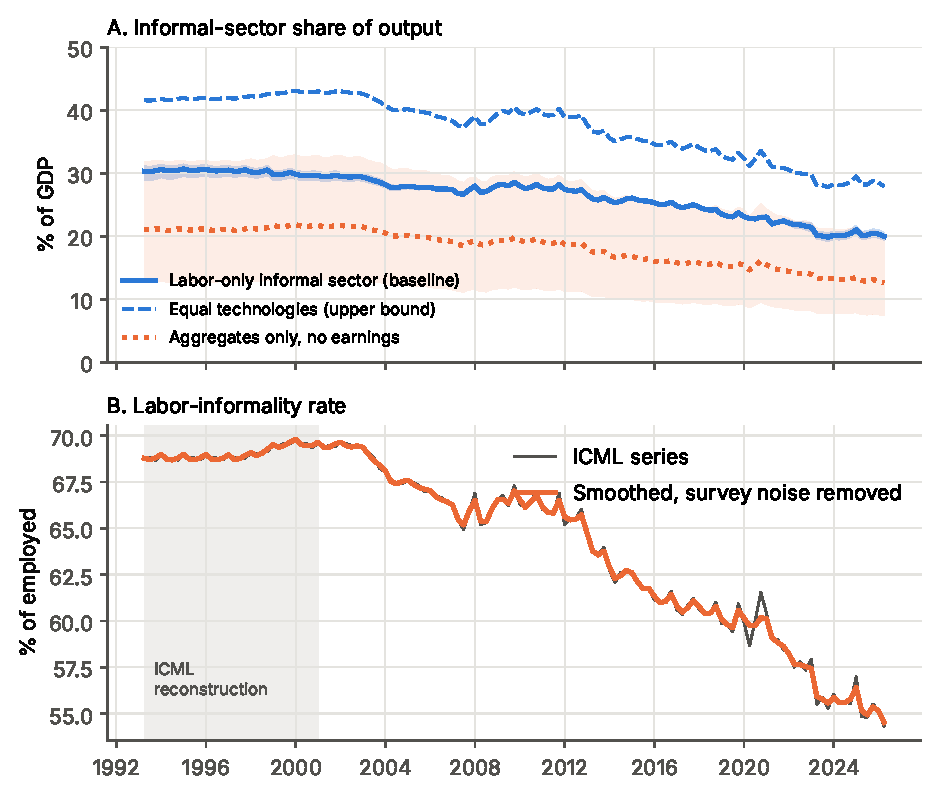
\includegraphics[width=0.9\textwidth]{fig_share_path.pdf}
\caption{Panel A: informal share of output, posterior median and 90\% band, baseline (labor-only informal sector, statutory non-wage costs), equal-technology estimate (upper bound) and estimate with aggregates only. Panel B: labor-informality rate from ICML and its smoothed value. The shaded area marks the ICML reconstruction (1993--2000).}
\label{fig:share}
\end{figure}

\subsection{Comparison with published estimates}
\label{sec:benchmarks}

Figure~\ref{fig:benchmarks} compares the estimate with the published annual series for Colombia included in our reference collection. Four families are available. The MIMIC estimates of Schneider and coauthors \citep{SchneiderBuehnMontenegro2010,MedinaSchneider2019} place the shadow economy at 36\%--40\% of official GDP in the 1990s and early 2000s and at 25\%--30\% after 2011. The enhanced MIMIC of \citet{AsllaniDellAnnoSchneider2024}, which restricts the concept to legal production deliberately concealed from the authorities, is almost flat at 24\%--27\%. The World Bank database \citep{ElginKoseOhnsorgeYu2021} reports a DGE series, built on the model of \citet{ElginOztunali2012}, that declines from 35\% in 1991 to 29\% in 2020, and a MIMIC series of 34\%--39\%. \citet{Vuletin2008} estimates 43.5\% for the early 2000s.

Published estimates differ among themselves by up to 19 percentage points in the same year, and the baseline lies inside that range throughout. It is 6 to 10 points below the MIMIC series of Schneider and coauthors between 1993 and 2005 and within about three points of \citet{MedinaSchneider2019} in 2008--2015, when that series falls to 25\%--31\%. It is within about one point of \citet{AsllaniDellAnnoSchneider2024} for 2009--2020, two to six points above it before and five below in 2021--2022. It is about six points below the World Bank DGE series in 2019--2020 and nine to fourteen below its MIMIC series. Its decline is steeper than that of the MIMIC series, which change little by construction. The equal-technology estimate lies at the top of the published range, next to \citet{Vuletin2008} and the World Bank MIMIC series, and the estimate without earnings below all of them.

\begin{figure}[H]
\centering
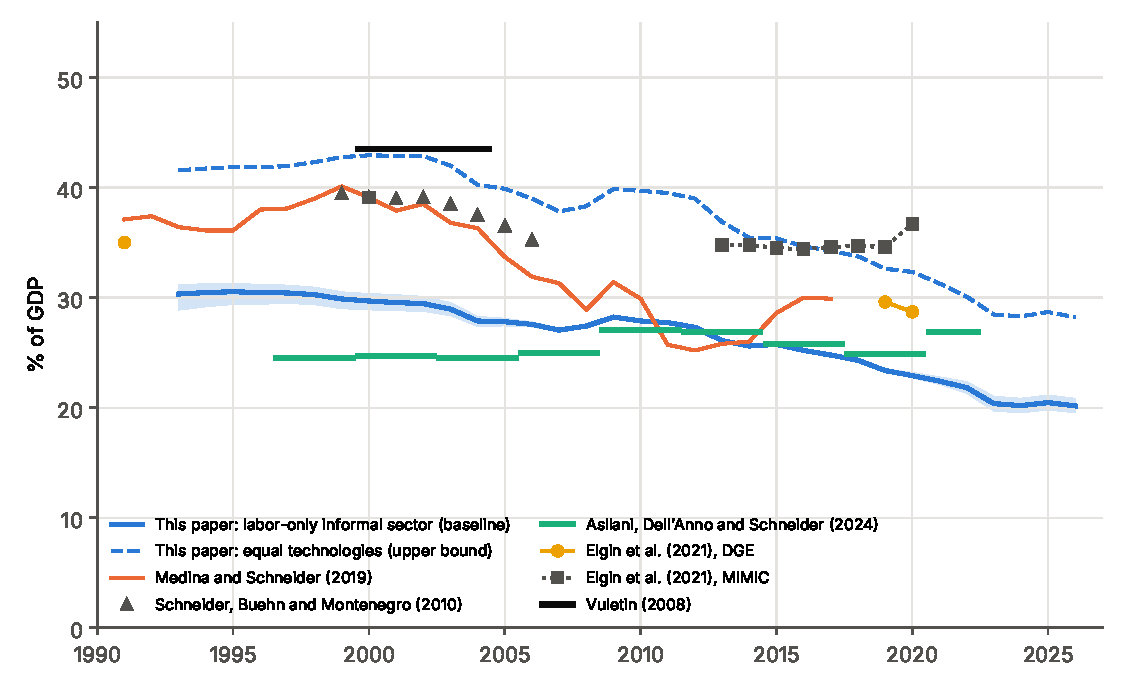
\includegraphics[width=0.9\textwidth]{fig_benchmarks.pdf}
\caption{Informal share of output: this paper and published estimates for Colombia (percent of GDP). Horizontal segments are period averages.}
\label{fig:benchmarks}
\end{figure}

Three differences in concept qualify the comparison. First, MIMIC estimates are expressed as a percentage of official GDP and treat the shadow economy as outside it, whereas the Colombian national accounts already include an estimate of the non-observed economy; our share is a fraction of measured GDP. Second, MIMIC levels are not independent measurements: they are converted to percentages of GDP with benchmark values from other studies, and \citet{AsllaniDellAnnoSchneider2024} anchor the scale to informal employment multiplied by an assumed informal wage, which is the accounting of Proposition~\ref{prop:share} with the earnings ratio assumed instead of measured. Third, our concept is the output of informal workers, which includes legal own-account production that is not concealed and excludes illegal activity. DANE's non-observed economy (22.4\% of gross production in the 2015 base) is not directly comparable either, because it refers to production rather than value added.

\subsection{Sensitivity}

The posterior bands reflect parameter and state uncertainty given the model and the measurement equation; uncertainty about the measurement assumptions is quantified by the sensitivity analysis. Table~\ref{tab:sensitivity} reports how the level changes with the concept of the formal wage (panel A), with other assumptions (panel B, around the constant-wedge specification) and with the technology (panel C). Three results stand out. First, the mapping from survey earnings to labor cost matters: with contributions only, the 2026 share is 22.8\% instead of 20.0\%, and with a constant 25\% wedge 20.6\%. Second, the capital share matters through the factor $1-\alpha$ in \eqref{eq:share}: with $\alpha=0.50$ the 2026 share is 17.0\% instead of 20.6\%. Third, the prior of $\eta$, the sample from 2007 and the capital--output ratio observed in levels leave the 2026 share within 0.2 points; observing capital raises the 1990s by about 3.5 points, because the model must accommodate the strong rise of the capital--output ratio in the sample. The equal-technology estimates bound the estimate from above.

\begin{table}[H]
\centering
\caption{Informal share of output under alternative specifications (posterior median and 90\% band, \%). $^{\dagger}$Largest $\hat R$ 1.053 (for $\theta$); the path is reported because it does not depend on $\theta$ (Table~\ref{tab:invariance}).}
\label{tab:sensitivity}
\scriptsize
\setlength{\tabcolsep}{4pt}
\begin{tabular}{l c c c c}
\toprule
\textbf{Specification} & $R$ & $\theta$ (steady state) & \textbf{1993Q2} & \textbf{2026Q2} \\
\midrule
\tableinput{tables/sensitivity.tex}
\bottomrule
\end{tabular}
\end{table}

The decline between 1993 and 2026, of ten to fifteen points, is common to every specification with earnings. Figure~\ref{fig:anchor} places the estimates on the mapping of Proposition~\ref{prop:share}.

\begin{figure}[H]
\centering
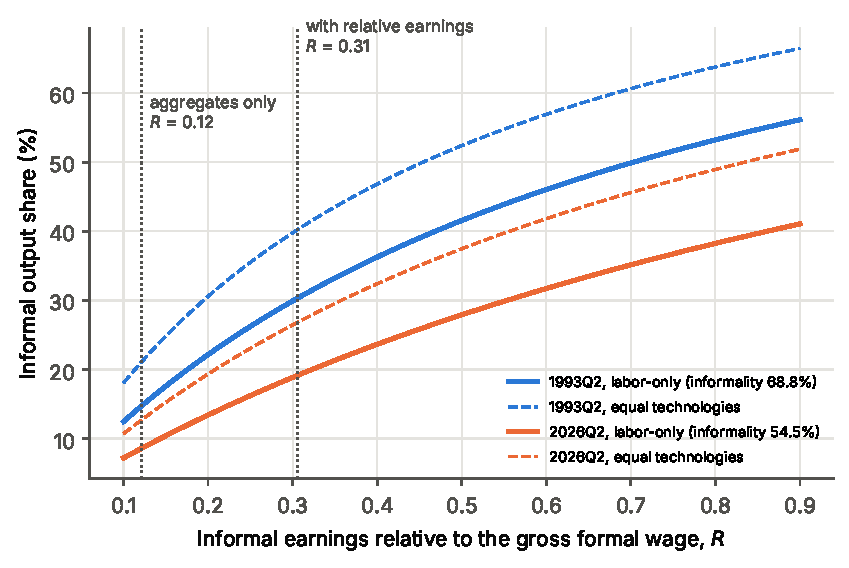
\includegraphics[width=0.75\textwidth]{fig_anchor_map.pdf}
\caption{Informal share of output implied by Proposition~\ref{prop:share} as a function of the earnings ratio $R$, at the informality rates of 1993Q2 and 2026Q2, for the labor-only and the equal-technology accounting. Dotted lines mark the posterior medians of $R$ with aggregates only and with the earnings observable.}
\label{fig:anchor}
\end{figure}

\section{Discussion: interpretation and implications}
\label{sec:discussion}

\subsection{What the estimate measures}

The estimate is the share of measured value added produced by informal work, as defined by the labor classification of the household survey. Proposition~\ref{prop:share} links it to three measurable quantities: the informality rate, relative earnings and the formal capital share. The link uses the survey concepts directly. The income of own-account workers and informal employers is mixed income, which already contains the return to their own capital, and the income of informal employees is adjusted by group (Section~\ref{sec:data}). The posterior bands report uncertainty given this mapping, and Table~\ref{tab:sensitivity} reports how the level moves under alternative mappings.

This concept is related to, but not the same as, the shadow or non-observed economy. Formal firms may employ workers informally, some own-account production is declared and included in the accounts, and illegal production is outside the labor classification used here. The comparisons in Figure~\ref{fig:benchmarks} are therefore checks of magnitude and trend. They are reassuring on both counts: the estimate lies within the range of published series, very close to the enhanced MIMIC estimates in 2009--2020, and shares their downward trend.

\subsection{Identifying the path}

The identification exercises separate two objects. The steady-state parameter $\theta$ is not pinned down by aggregate data, which explains why calibrated and estimated DGE models in the literature can reach very different levels for the same country. The quarterly path of the informal share, which is the object of interest, is identified once relative earnings are observed: from 2007 it is pinned down by the observed informality rate, the observed earnings ratio and the capital share, and it is invariant to $\theta$ within 0.3 percentage points. Before 2007 the path is identified with the information available for those years, the reconstructed informality rate and the national accounts, and the model carries the earnings information back; this step moves the 1990s by at most 1.4 points across values of $\theta$ between 0.10 and 0.40. Simulations with known parameters recover the true share with high precision.

The practical implication for this literature is that the level of the informal economy in a DGE model should be identified by a direct measure of relative productivity rather than by the aggregates or by calibration, and that the identification check should be reported together with the posterior.

\subsection{Implications for research and policy}

The estimates show that the contribution of informal work to output has declined together with labor informality, from about 30\% to 20\% of GDP over three decades. They also quantify the productivity gap behind the difference between the two measures: at the end of the sample informal value added per worker is about one-fifth of formal value added per worker. This gap is the relevant magnitude for policy discussions. Formalizing a worker does not by itself raise output; what matters is whether the worker moves into higher-productivity activity. Evaluating specific reforms, such as changes in payroll taxes or enforcement, is a natural next step for the model, which already contains the formality wedge through which such policies operate.

Because the data and code are public and the earnings series is built from the regular household survey, the estimate can be updated every quarter. It thus offers a timely complement to DANE's periodic measurement of the non-observed economy.

\section{Scope and extensions}
\label{sec:limitations}

The estimates rest on choices made with the information available. Each of them is explicit and testable, and each points to an extension that would sharpen the results.

\paragraph{From earnings to value added.} The baseline treats the mixed income of own-account workers and employers as their value added and adjusts the earnings of informal employees by group. The sensitivity analysis shows how much the level depends on this treatment, and the equal-technology specification bounds it from above. Direct data on the value added and capital of informal units, such as DANE's micro-business survey (EMICRON), would allow this mapping to be estimated rather than assumed.

\paragraph{Labor costs and the capital share.} Formal labor costs are computed from the statutory non-wage costs; actual payments may differ because of exemptions or noncompliance. With contributions only, the 2026 share is 22.8\% instead of 20.0\%. The capital share, $\alpha=0.354$, is estimated from Colombian data and agrees with the GRECO historical accounts (0.36--0.42); a value of 0.50 lowers the 2026 share to 17\%. Firm-level labor-cost data and sectoral capital-share estimates would narrow this range.

\paragraph{The historical period.} Before 2007 there are no consolidated microdata on informal earnings, and the national-accounts and labor-market series for the 1990s are reconstructions. The paper uses all the information that exists for those years, and the invariance and sensitivity results show how much the early path depends on the model. Any future recovery of historical survey microdata could enter the estimation directly, since the Kalman filter handles missing observations.

\paragraph{Model structure.} A representative labor-only informal technology summarizes a heterogeneous sector of own-account workers, employees of unregistered units and informally hired workers in registered firms. Splitting the informal sector by type of worker, and adding observed policy instruments to the formality wedge, would allow the model to be used for policy evaluation.

None of these choices alters the main results: the accounting relationship, the identification of the path by relative earnings, and the decline of the informal share from about 30\% to 20\% of GDP.

\section{Conclusions}
\label{sec:conclusions}

This paper estimates the contribution of informal work to Colombian output from 1993 to 2026. In a two-sector DSGE model, the informal output share depends on three quantities: the proportion of workers employed informally, their value added per worker relative to formal workers, and the capital share of formal production. The first is observed in the informality rate, the second is measured with a new quarterly series of relative earnings built from household-survey microdata, and the third is estimated from Colombian data.

The identification analysis shows why the relative-earnings series is needed. Aggregate national accounts and labor-market series do not determine the size of the informal sector on their own: likelihood profiles, prior--posterior comparisons and simulations with known parameters all point in that direction. With relative earnings, the quarterly path of the informal share is identified, invariant to the model's steady state and recovered precisely in simulations. The distinction between the path, which the data identify, and the steady-state parameter, which they do not need to identify, is the key to estimating the informal economy with a DSGE model.

Under the baseline specification, the informal share falls from about 30\% of GDP in 1993 to 20\% in 2026Q2, while labor informality falls from about 69\% to 54\%. Informal value added per worker is about one-fifth of formal value added per worker, which explains how a majority of workers can be informal while producing a fifth of output. The estimates lie within the range of published Colombian series and close to the most recent MIMIC estimates.

The model delivers more than the informal share: quarterly informal and formal GDP, relative productivity, the informality rate net of measurement error and the structural shocks behind them, all of which are published with the paper. The data and code allow the series to be updated every quarter and extended as new information becomes available, in particular direct measures of the value added of informal units and observed policy instruments that would turn the model into a tool for evaluating formalization policies.


\section*{Ethical Statement}

This study uses aggregated official statistics, a public research dataset derived from them, and the anonymized public-use microdata of DANE's household survey (GEIH), from which only quarterly aggregates are computed. The analysis uses no directly identifying survey records and involves no contact with research participants. Ethics-review requirements, if any, remain subject to the author's institutional rules.

\section*{Acknowledgments}

The author acknowledges the work of the Departamento Administrativo Nacional de Estad\'istica (DANE) in producing and publishing the statistics on which this study relies. The views and conclusions expressed here are solely those of the author. The results are research estimates and are not official statistics.

\section*{Funding and Competing Interests}

This research received no funding from public agencies, private institutions or nonprofit organizations. The author declares no competing interests.

\section*{Data and Code Availability}

The labor series are those of ICML release 2.6.1, archived at \url{https://doi.org/10.5281/zenodo.24357243}. The GEIH microdata are published by DANE in its microdata catalog. The quarterly dataset used in the estimation, the relative-earnings series, the script that computes it from the GEIH microdata, the estimation code (model, state space, sampler, diagnostics and the earnings measurement equation), the result files and the script that regenerates the figures and tables are distributed as ancillary files of this paper.


\bibliographystyle{plainnat}
\bibliography{references}

\appendix
\section{The model in detail}
\label{app:model}

This appendix lists the equations exactly as they are solved and estimated. The code that implements them is in the ancillary files (\code{m2/model.py} and \code{m2/statespace.py}).

\subsection{Stationary equilibrium conditions}

Let $c_t=C_t/X_t$, $y_t=Y_t/X_t$, $y_{f,t}=Y_{f,t}/X_t$, $y_{i,t}=Y_{i,t}/X_t$, $i_t=I_t/X_t$, $g_t=G_t/X_t$, and $k_t=K_t/X_{t-1}$. Capital per unit of the current trend is $\tilde k_t = K_t/X_t = k_t\,e^{-(\gamma+\mu_t)}$. The thirteen equations, in the order of the code, are:
\begin{align}
&\text{(1) Output:} && y_t = y_{f,t} + y_{i,t},\quad y_{f,t}=\tilde k_t^{\alpha}N_{f,t}^{1-\alpha},\quad y_{i,t}=A_i e^{z^r_t}N_{i,t}^{\eta} \\
&\text{(2) Formal labor:} && \psi_t\chi_fN_{f,t}^{\varphi}c_t = (1-\bar\tau)e^{-\omega_t}(1-\alpha)\,y_{f,t}/N_{f,t} \\
&\text{(3) Informal labor:} && \psi_t\chi_iN_{i,t}^{\varphi}c_t = \eta\,y_{i,t}/N_{i,t} \\
&\text{(4) Resources:} && y_t(1+\bar x + x_t) = c_t + i_t + g_t,\quad g_t=\bar g\,e^{z^g_t} \\
&\text{(5) Capital:} && k_{t+1} = (1-\delta)\tilde k_t + \nu_t i_t \\
&\text{(6) Euler:} && \frac{1}{\nu_tc_t} = \beta E_t\Big[\frac{e^{-(\gamma+\mu_{t+1})}}{c_{t+1}}\Big(\alpha\frac{y_{f,t+1}}{\tilde k_{t+1}} + \frac{1-\delta}{\nu_{t+1}}\Big)\Big] \\
&\text{(7)--(13) Shocks:} && \zeta_{t+1}=\rho_\zeta\zeta_t+\sigma_\zeta\varepsilon_{\zeta,t+1},\quad \zeta\in\{\mu, z^g,\ln\nu,\ln\psi,\omega,x,z^r\}
\end{align}
The factor $e^{-(\gamma+\mu_{t+1})}$ in the Euler equation appears because $C_{t+1}=c_{t+1}X_{t+1}$ and $X_{t+1}=X_te^{\gamma+\mu_{t+1}}$: a positive trend shock raises future consumption and lowers its marginal utility. In equation (5), capital installed in $t$ is divided by $X_t$ and becomes $k_{t+1}$.

\subsection{Steady state}

At $\zeta_t=0$ for every shock and with the calibration of Table~\ref{tab:calibration}:
\begin{align*}
r &= e^{\gamma}/\beta-1+\delta, & \tilde k/y_f &= \alpha/r, & N_f &= \bar N(1-\bar s),\quad N_i=\bar N\bar s,\\
y_f &= (\tilde k/y_f)^{\alpha/(1-\alpha)}N_f, & y &= y_f/(1-\theta), & y_i&=\theta y,\quad A_i = y_i/N_i^{\eta},\\
k &= e^{\gamma}\tilde k, & i &= k-(1-\delta)\tilde k, & c &= (C/Y)\,y,\quad g=(G/Y)\,y,\\
\bar x &= (c+i+g)/y-1, & \chi_f &= \frac{(1-\bar\tau)(1-\alpha)y_f/N_f}{N_f^{\varphi}c}, & \chi_i &= \frac{\eta\,y_i/N_i}{N_i^{\varphi}c}.
\end{align*}
The steady-state earnings ratio that enters the measurement equation is
\[
\bar R = \frac{y_i/N_i}{(1-\alpha)\,y_f/N_f} = \frac{\theta}{(1-\theta)(1-\alpha)}\cdot\frac{1-\bar s}{\bar s},
\]
which is Proposition~\ref{prop:share} inverted at the steady state. At the posterior median ($\theta=0.277$, $\alpha=0.354$, $\bar s=0.645$) it is 0.33.

\subsection{Linearization and solution}

Let $\bm{z}_t$ be the vector of the thirteen variables in logarithms (shocks in levels) and $\bar{\bm{z}}$ its steady state. Writing the system as $\bm{f}(\bm{z}_t, E_t\bm{z}_{t+1})=\bm{0}$, the first-order approximation is
\[
\bm{F}_1\,(\bm{z}_t-\bar{\bm{z}}) + \bm{F}_2\,E_t(\bm{z}_{t+1}-\bar{\bm{z}}) = \bm{0},
\]
where $\bm{F}_1$ and $\bm{F}_2$ are the Jacobians with respect to current and expected future values, computed by central finite differences. The generalized Schur (QZ) decomposition of the pencil $(-\bm{F}_1,\bm{F}_2)$ is ordered so that stable eigenvalues come first \citep{Klein2000}. With eight stable eigenvalues for eight states the solution is unique and takes the form \eqref{eq:solution}; otherwise the parameter draw is rejected. The solution is checked by verifying that $\bm{F}_1\bm{M} + \bm{F}_2\bm{M}\bm{T} = \bm{0}$, where $\bm{M}$ maps the states into all variables.

\subsection{Measurement equations}

Hats denote log deviations from the steady state and $q(t)$ the quarter of the year. The observables of the baseline are linked to the model as follows.
\begin{align*}
\Delta\ln Y^{\mathrm{obs}}_t - m^{Y}_{q(t)} &= \hat y_t - \hat y_{t-1} + \mu_t + u^Y_t,\\
\Delta\ln C^{\mathrm{obs}}_t - m^{C}_{q(t)} &= \hat c_t - \hat c_{t-1} + \mu_t + u^C_t,\\
\Delta\ln I^{\mathrm{obs}}_t - m^{I}_{q(t)} &= \hat\imath_t - \hat\imath_{t-1} + \mu_t + e^I_t - e^I_{t-1} + u^I_t,\\
\Delta\ln G^{\mathrm{obs}}_t - m^{G}_{q(t)} &= z^g_t - z^g_{t-1} + \mu_t + u^G_t,\\
\Delta\ln N^{\mathrm{obs}}_t - m^{N}_{q(t)} &= (1-\bar s)(\hat n_{f,t}-\hat n_{f,t-1}) + \bar s(\hat n_{i,t}-\hat n_{i,t-1}) + e^N_t - e^N_{t-1} + u^N_t,\\
\logit s^{\mathrm{obs}}_t - \logit\bar s - \kappa_{q(t)} &= \hat n_{i,t} - \hat n_{f,t} + e^s_t,\\
\ln R^{\mathrm{obs}}_t - \ln\bar R
&= \ln(1+d_t^{\mathrm{nw}}) + b\,\mathbb{1}_{t\ge2022Q1}
  + z^r_t + (\eta-1)\hat n_{i,t} \\
&\quad - \alpha(\hat k_t - \mu_t - \hat n_{f,t}) + e^R_t .
\end{align*}
The trend shock $\mu_t$ appears in the growth rates because detrended variables are measured relative to $X_t$, whose growth is $\gamma+\mu_t$; the mean growth $\gamma$ is removed with the quarter-of-year means $m_q$. Total employment is linearized as a weighted average of the two types of work. The errors $e^I$, $e^N$ are level errors carried as states, $e^s$ and $e^R$ are independent errors of the two observables in levels, and $u$ is the small growth-rate error that keeps the covariance of the observables non-singular. $\kappa_q$ is the quarter-of-year pattern of the logit informality rate over 2005--2018, centered at zero. In the last equation, $\ln(1+d_t^{\mathrm{nw}})$ converts the wages reported in the survey into the employer's labor cost.

\subsection{Likelihood and sampler}

Stacking the states of \eqref{eq:solution}, their lags and the level errors in a vector $\bm{\xi}_t$, the model and the measurement equations form a linear Gaussian state-space system,
\[
\bm{\xi}_{t+1} = \bm{A}\bm{\xi}_t + \bm{B}\bm{\varepsilon}_{t+1},\qquad \bm{y}^{\mathrm{obs}}_t = \bm{Z}\bm{\xi}_t + \bm{u}_t .
\]
The Kalman filter computes, quarter by quarter, the forecast of the observables given the past, the forecast error $\bm{v}_t$ and its covariance $\bm{F}_t$, and the log likelihood is $-\tfrac12\sum_t\big(\ln|2\pi\bm{F}_t| + \bm{v}_t^{\top}\bm{F}_t^{-1}\bm{v}_t\big)$ over the observed entries. Quarters with missing observations use only the entries that are observed. The posterior is the likelihood times the prior; the random-walk Metropolis--Hastings sampler proposes a new parameter vector near the current one and accepts it with probability $\min\{1, p(\text{new})/p(\text{current})\}$, so that after a burn-in the accepted draws are a sample from the posterior. The Kalman smoother then recovers, for each draw, the path of the states given all the data, from which the informal share of output \eqref{eq:share} is computed.


\end{document}
